\documentclass[a4paper]{article}
\usepackage[warn]{mathtext}
\usepackage[utf8]{inputenc}
\usepackage[T2A]{fontenc}
\usepackage[english,russian]{babel}
\usepackage{indentfirst}
\usepackage{misccorr}
\usepackage{subcaption}
\captionsetup{compatibility=false}
\usepackage{geometry}
\geometry{verbose,a4paper,tmargin=2cm,bmargin=2cm,lmargin=1.5cm,rmargin=1.5cm}
\usepackage{graphicx}
\usepackage{wrapfig}
\usepackage{amsmath}
\usepackage{fancyhdr}
\usepackage{floatflt}
\usepackage{float}
\usepackage{amssymb}
\usepackage{color}
\usepackage{lscape}
\usepackage{hvfloat}
\usepackage{amsfonts}
\usepackage{euscript}
\usepackage{newunicodechar}
\usepackage{booktabs}
\usepackage{epigraph}
\usepackage{csquotes} 
\usepackage{hyperref}

\hypersetup{
    colorlinks=true,      
    urlcolor=blue,
    linkcolor= blue
}

\begin{document}
\newcommand{\apple}{\char"F8FF}



\begin{titlepage}
    \vspace*{4cm}
	\centering
    {\scshape\LARGE Московский физико-технический институт\par}
	\vspace{1cm}
	{\scshape\Large Эсее по защите информации\par}
	\vspace{1cm}
    {\huge\bfseries  Криптрографические протокол Girault\par}
	\vspace{2cm}
	\vfill
\begin{flushright}
	{\large Выполнила студентка Б01-907}\par
	\vspace{0.3cm}
	{\LARGE Юлия Прохорова}
\end{flushright}
	
	\vfill
Долгопрудный, 2022
% Bottom of the page
\end{titlepage}

\pagestyle{fancy} 
\fancyhead[L]{Криптографические протокол Girault}
\fancyhead[R]{Юля Прохорова, Б01-907}
\fancyhead[C]{}
\fancyfoot[C]{ \noindent\rule{\textwidth}{0.4pt} \thepage }

\tableofcontents

\newpage

\epigraph{Кто владеет информацией, тот владеет и миром.}{Натан Майер Ротшильд}

\section{Введение}
Криптографию назвают наукой или даже искусством безопасных сообщений называется. Криптография встречается и в повседневной жизни, например, суметь помешать прочитать ваш личный дневник, зашифровав его особым образом. Но здесь мы поговорим о криптографии, которая защищает важные файлы, документы или банковские счета от любого, кто попытается их прочесть.
  \par
  \begin{displayquote}
    Брюс Шнайер пишет: "Если я беру письмо, кладу его в сейф где-нибудь в Нью-Йорке, затем велю Вам прочитать это письмо, то это не безопасность. Это непонятно что. С другой стороны,
  если я беру письмо и кладу его в сейф, затем передаю этот сейф Вам вместе с детальным описанием, передаю также сотню подобных сейфов
  с их комбинациями, чтобы Вы и лучшие "медвежатники мира" могли изучить систему замков, а вы все равно не сможете открыть сейф 
  и прочитать письмо - вот это и есть безопасноть." 
 \end{displayquote}
 
 Современная криптография - общирная область знаний, сложившаяся в результате серьезных исследований на протяжении последних десятков лет. 
 \par 
 Данная работа направлена на то,
  чтобы познакомить читателя с криптографическими протоколами,а именно с протоколом Girault. Но не обо всем сразу. Начнем с сновных понятий и терминов.

\section{Общая теория}

Обычная ситуации при изучении криптографии - две стороны: отправитель и получатель, и первый хочет послать сообщение второму. При этом отправлять сообщение необходимо безопасным образом -  чтобы перехвативший не мог его прочесть. \par
В данном случае само сообщение будет называться \textbf{открытым текстом}. Изменение сообщения так, чтобы не была понятна его суть - это \textbf{шифрование}, полученный текст - \textbf{шифротекст}.
\textbf{Дешифрованием} же называется процесс преобразования шифротекста в открытый текст.

\textbf{Шифр}(или криптографический алгоритм) представляет собой математическую функцию, используемая для шифрования и дешифрования.

\subsection{Протоколы}
\textbf{Протокол} - порядок действий, предпринемаемых сторонами, чтобы решить поставленную задачу. Каждое действие должно выполняться в свою очередь и только
после окончания предыдущего.
\par
Каждый протокол должен обладать следующими характеристиками:
\begin{itemize}
    \item Известность - каждый участник протокола должен знать протокол и последовательность составляющих его действий;
    \item Cогласованность - каждый участник протокола должен согласиться следовать ему;
    \item Отсутствие противоречий (прозрачность) - каждое действие должно быть определено так, чтобы не было возможности непонимания;
    \item Полнота -  каждой ситуации соответствует определенное заранее действие.
\end{itemize}

Криптографический протокол выходит за рамки одной лишь безопасности, участники протокола могут:
\begin{itemize}
    \item Поделится секретом друг с другом;
    \item Случайно сгенерировать случайную последовательность;
    \item Подтвердить свою подлинность или подписать контракт одновременно.
\end{itemize}

Для демонстрации работы протоколов обычно обозначают его участников: Alice - начинает протокол, Bob - отвечает, также при необходимости третьих сторон появляются Carol и Dave.
\par 
Далее рассмотрим основные виды протоколов: \par
\subsubsection*{Протокол с посредником}
Посредник - незаинтересованная 3я сторона, которая завершает протокол. При этом все участники протокола принимают за истину все, что скажет посредник. Все его действия - правильные, и все стороны протокола уверены в том, что посредник выполнит свою часть протокола.
\par такой вид протоколов предназначен для взаимодействия недоверяющих друг другу сторон.

У данного протокола, как и любого другого существуют недостатки:
\begin{itemize}
    \item Сложно доверять безликому посреднику
    \item Компьютерная сеть должна обеспечить поддержку посредника
    \item Задержка
    \item Посредник должен принимать участие в каждой транзакции, являясь узким местом ы крупномасштабных реализациях протокола.
    \item Так как каждый участник протокола должен доверять посреднику, то посредник может стать слабым местом сети при попытке ее взлома.
\end{itemize}
\subsubsection*{Арбитражные протоколы}
Арбитражный протокол делится на два подпротокола: один представляет из себя протокол без посредника - он выполняется, если стороны смогл самостоятельно договориться, второй - протокол с посредником, которого приглашают в случае разногласия между сторонами (здесь посредника называют арбитром).
\par 
Арбитр - это незаинтересованное лицо, участвующее в протоколе, которому доверяют обе стороны. Его приглашают для проверки честности выполнения протокола между сторонами.
Хороший арбитражный протокол может не только определить факт мошенничества, но также и определить сторону, которой были совершены злодеяния. Такой протокол лишь обнаруживает мошенничество, но не предсказывает и не предотвращает его.
\subsubsection*{Самодостаточные протоколы}
Такие протоколы называются лучшими, так как они обеспечивают полную честность сторон. Здесь не требуется посредники, даже в критические моменты, как в арбитражных протоколах. Протокол построен так, что при попытке смошенничать одной стороны - другая сразу узнает об этом, а протокол прекращает выполняться.
Главный минус такого протокола состоит в том, что не сущетсвует такого самодостаточного протокола, который подходил бы под все ситуации. 
\subsubsection*{Попытки вскрытия протоколов}
Существует много способов взломать протокол. Можно просто подслушивать протокол, пробуя добыть информацию - это \textbf{пассивное вскрытие}, так как взломщик никак не воздействует на сам протокол.
Такой тип взлома относится к взлому с использованием шифротекста. Такой вид взлома сложно обнаружить, поэтому протоколы стараются предотвратить их.

Другой способ - \textbf{активное вскрытие }, по сути - просто изменение протокола. Например, можно попробовать подменить сообщение, повторное оправить старое или внести новое.
Пассивные взломщики занимаются сбором информации и криптоанализом сообщений. Активные взломщики стараются получить доступ к ресурсам или ухудшить работу системы.
Взломщиком может оказаться, кто угодно - даже участник протокола. Он может обманывать, выполняя протокол или наоборот не следовать протоколу вовсе. Такой взломщик - мошенник. Пассивные мошенники выполняют правила протокола, но стараютсяполучить больше информации, чем предусмотренно протоколом.
Активные нарушают работу протокола.
\subsection{Распространение ключей}
Для того чтобы создать и настроить надежную сеть необходимо безопасно распределять ключ - так, чтобы два конечных пользователя могли в одновременно получить секретный сессионный ключ шифрования. \\
Вот параметры, по которым определяют качество качество протокола распространения ключей:
\begin{itemize}
    \item Результатом работы протокола является - секретный сессионный ключ.
    \item Окончание протокола подразумевает под собой - успешную взаимную аунтефикацию абонентов.
    \item Внешний пользователь не должен иметь возможность получить общий сессионный ключ с кем-то из внутренних пользователей.
    \item Добавление и удаление участников из сети производится без уведомления всех участников сети.
\end{itemize}
Сети бывают с выделенным доверенным центром и без. Второй вариант плох тем, что с ростом количества участников сети, количество пар мастер-ключей растет с квадратичной скоростью.
\begin{figure}[H]
	\begin{center}
	\begin{minipage}[h]{0.45\linewidth}
	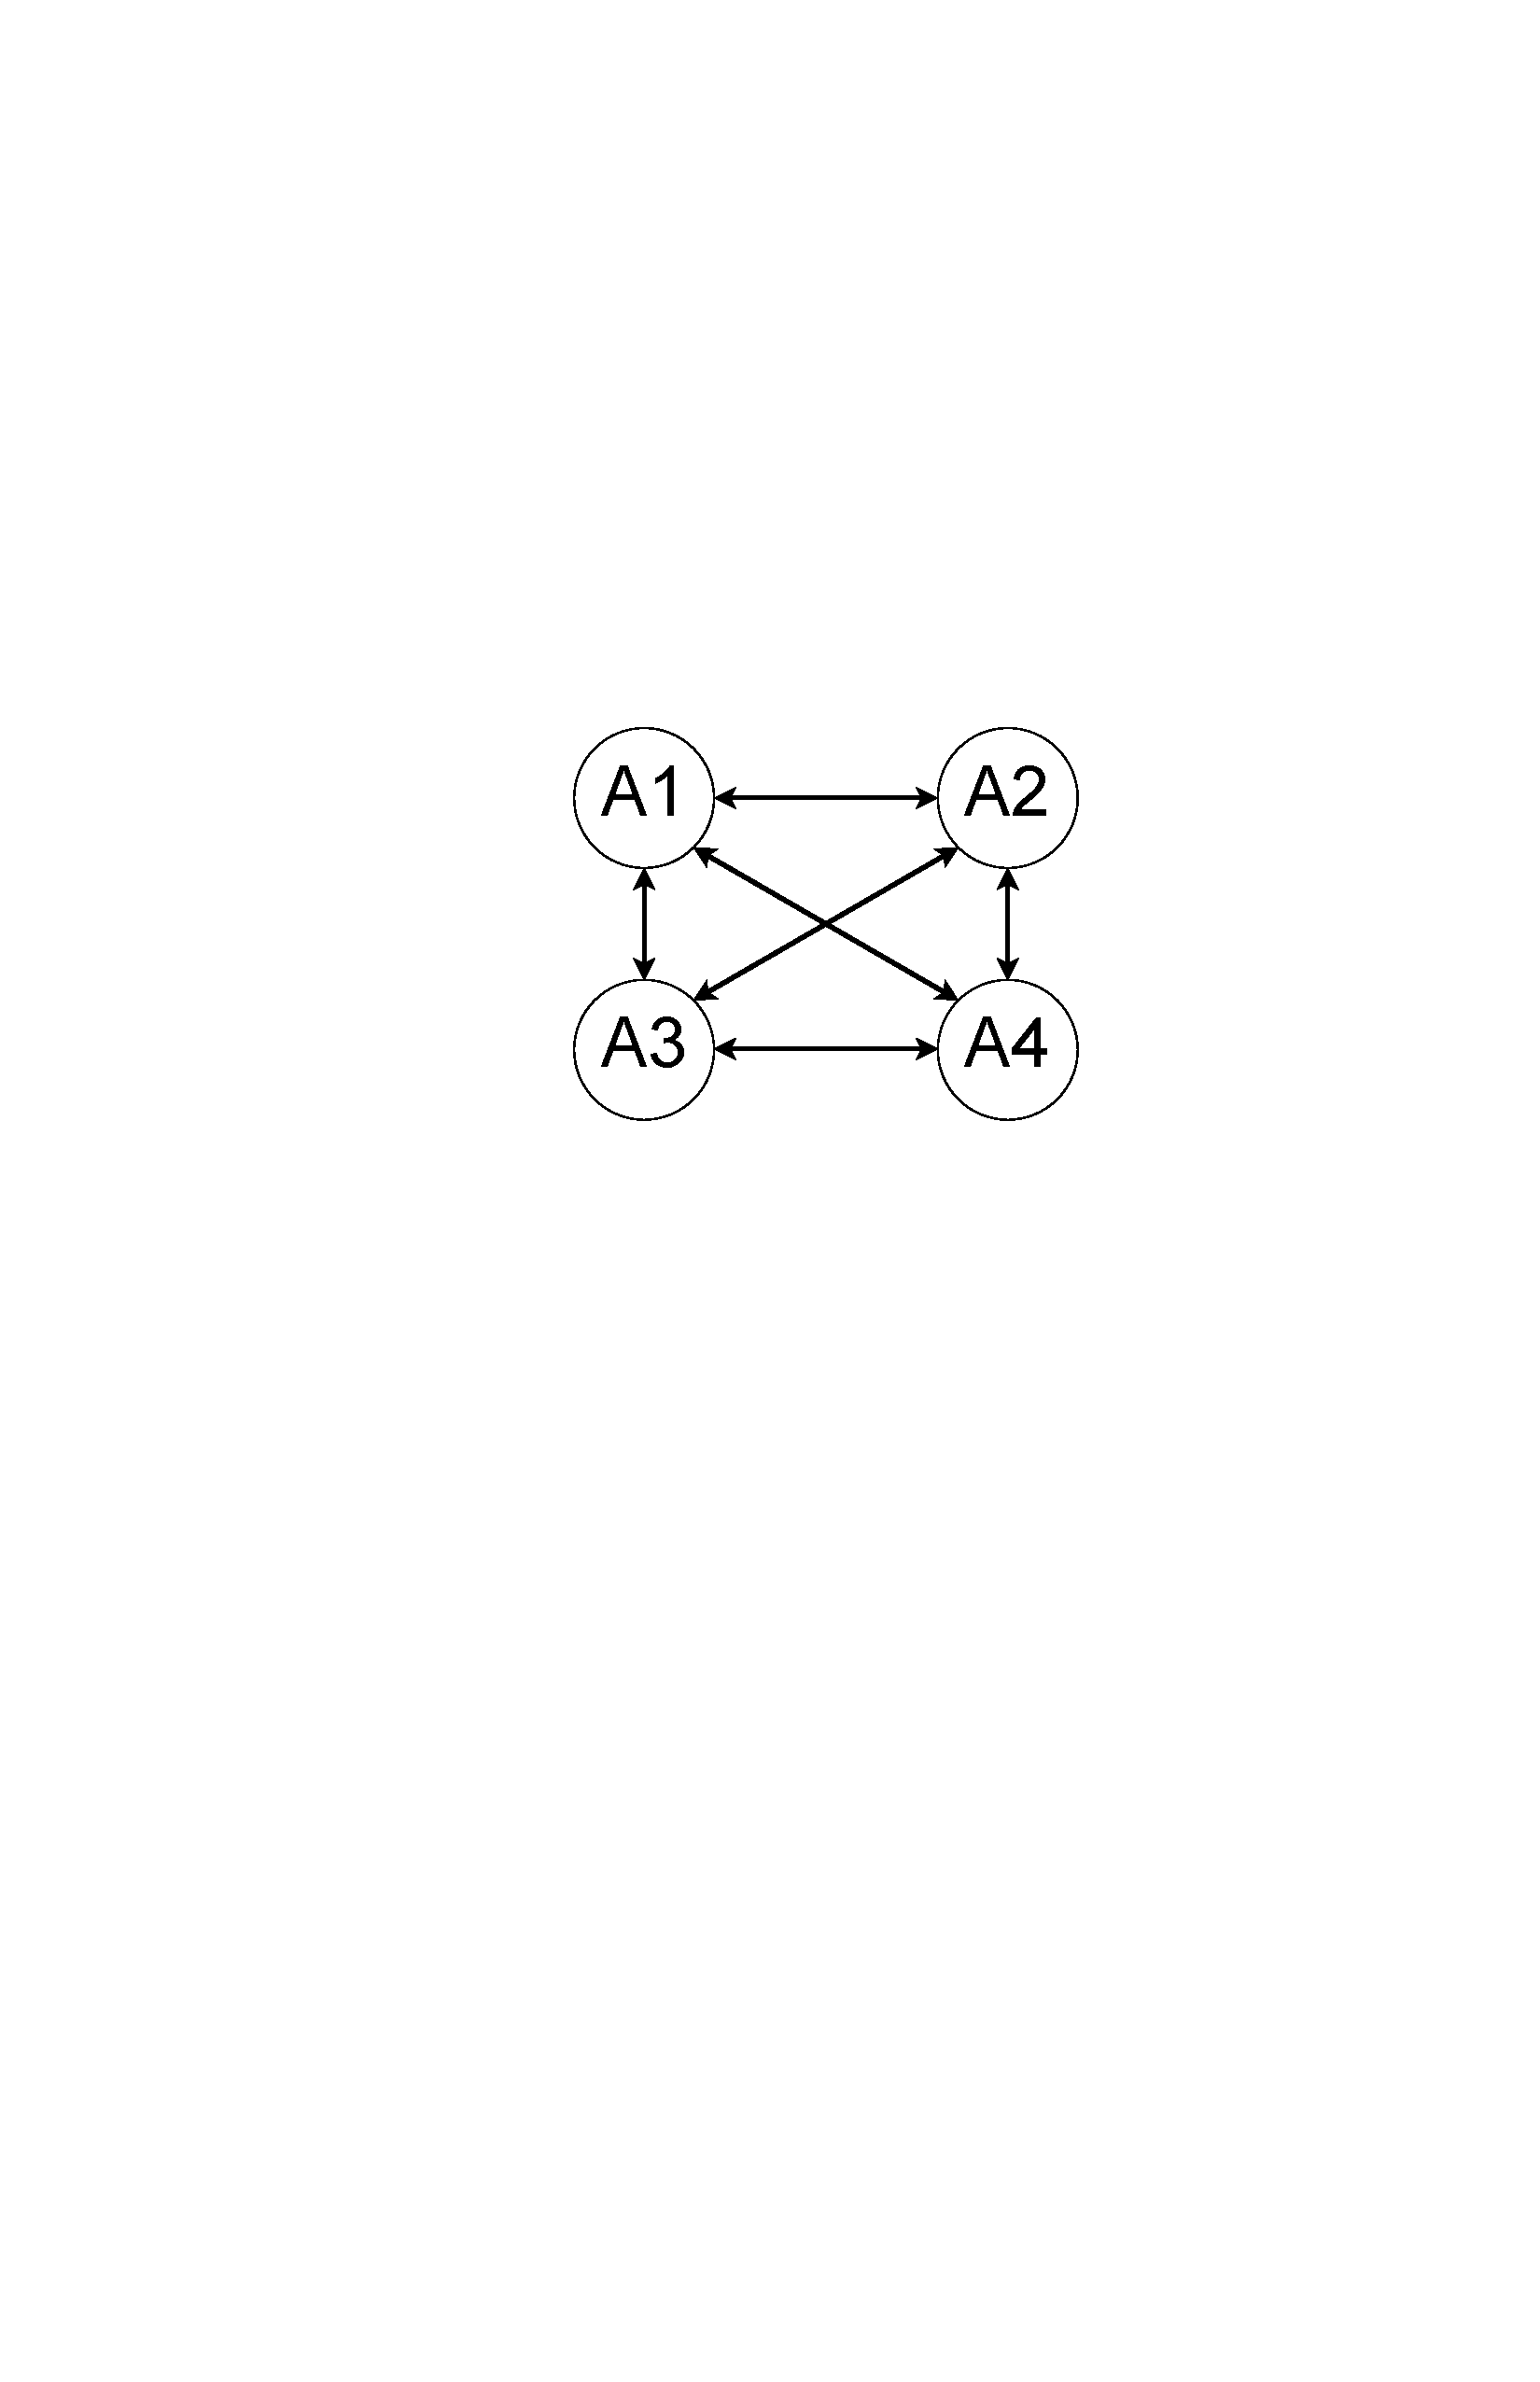
\includegraphics[width=1\linewidth]{pic1.pdf}
	\caption{Сеть без выделенного доверенного центра.} 
    \label{p2}
	\end{minipage}
	\hfill 
	\begin{minipage}[h]{0.43\linewidth}
	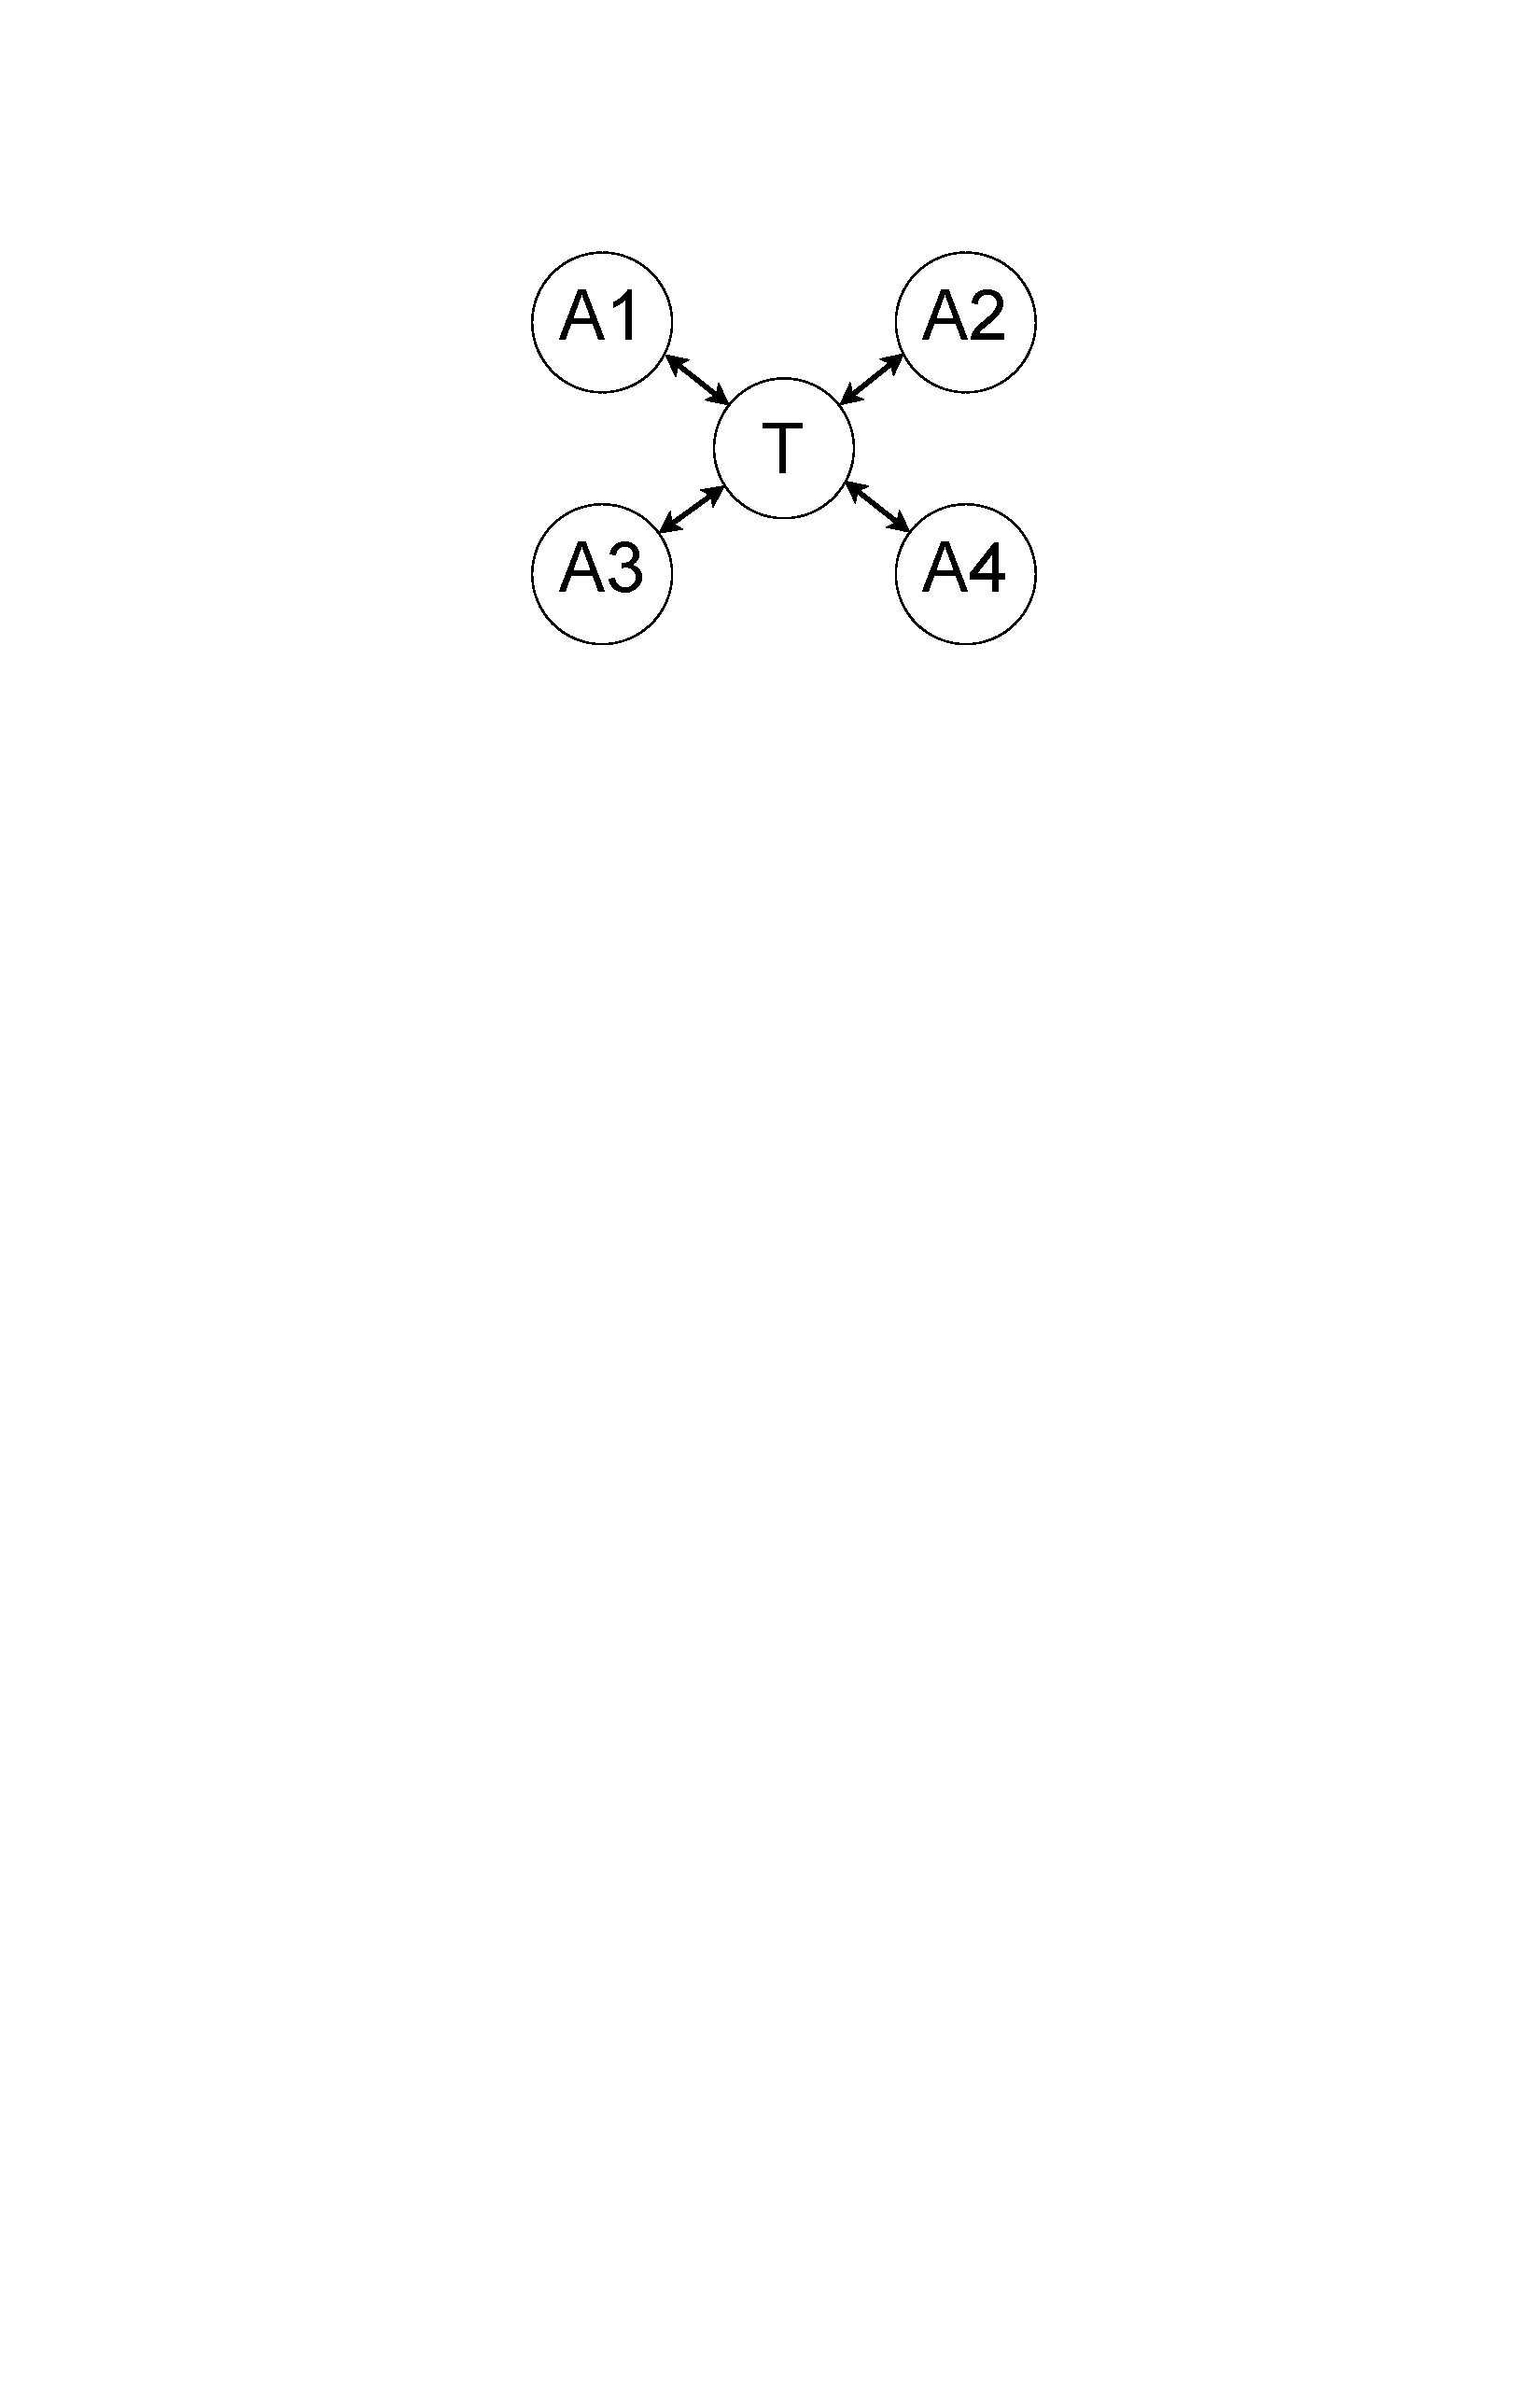
\includegraphics[width=1\linewidth]{pic2.pdf}
	\caption{Сеть с выделенным доверенным центром.}
	\label{p3}
	\end{minipage}
	\end{center}
\end{figure}

Протокол распространения ключей должен реализовывать следующие цели:
\begin{itemize}
    \item Аунтефикация сторон протокола;
    \item Защита от повтора;
    \item Аунтефикация ключа;
    \item Подтверждение владения ключом;
    \item Совершенная секретность;
    \item Формирование новых ключей;
    \item Ограниченная ащита от атак каза в обсуживании.
\end{itemize}

Изучим более подробно схемы распределения ключей с доверенным центром на примере протокола Жиро. 
Но для начала рассмотрим этапы:
\begin{enumerate}
    \item Доверенный центр создает секрет, известный только ему.
    \item Для каждого нового участника сети доверенный центр, используя секрет, вырабатывает сертификат, который позволяет новому участнику 
    вырабатывать сеансовые ключи с другими участниками.
    \item Начинается общение участников. Они предъявляют друг другу идентификаторы от доверенного центра. Далее используя эту информацию они могут сгенерировать секретный сеансовый ключ для общения мужду собой.
\end{enumerate}

\section*{Протокол Girault}

\textbf{Протокол Жиро} (фр. Marc Girault) — криптографический протокол, позволяющий двум сторонам получить общий секретный ключ, не используя явную сертификацию (схема распределения ключей с доверенным центром). 
Полученный ключ используется для шифрования дальнейшей обмениваемой информации с помощью симметричного шифрования.

Схема распределения ключей, предложенная Жиро в 1991, решает проблему ранних протоколов, основанных на удостоверении личности,
 в которых стороны выбирают свои секретные ключи заключалась в том, что пользователи используют свои личные данные
  для формирования новых скрытых сертификатов. Так как верификатор и пользователь могут образовывать противоречивые 
  свидетельства, то не возможно определить, кто из них может быть злоумышленником, когда появляются два сертификата.

Жиро решил эту проблему путём определения ключа, который сам себя сертифицирует. 
Схема Жиро предполагает участие доверенного Трента, с которым пользователи могут обмениваться информацией 
по надёжному защищённому каналу. Только доверенный Трент может генерировать скрытую сертификацию для этих ключей.

В схеме Жиро пользователь может сам выбрать свой закрытый ключ. Надёжность схемы Жиро строится на стойкости криптосистемы 
RSA (сложности факторизации больших чисел и вычисления дискретного корня).
\\
Опишем общий алгоритм:
\begin{enumerate}
    \item Доверенный центр Т:
    \begin{enumerate}
        \item выбирает оббщий модуль $n = p \cdot q$, где $p$ и $q$ - большие простые числа;
        \item выбирает пару из закрытого $(d,n)$ и открытого $(e,n)$ ключей; 
        \item выбирает элемент g поля $Z_n^\times$ максимального порядка;
        \item публикует в открытом доступе для участников параметры: n, e, g.
    \end{enumerate}
    \item Участники:
    \begin{enumerate}
        \item выбирают себе закрытый ключ s (каждый свой) и идентификатор;
        \item вычисляет и отправляет доверенному центру $v = g ^{-s} mod n$;
        \item используя протокол аунтефикации сторон участник доказывает доверенному центу Т, что владеет закрытым ключом, не раскрывая его значение;
        \item получает от доверенного центра свой открытый ключ $P = (v - I)^d = (g^{-s} -I)^d mod n$;
    \end{enumerate}
    \item в результате для каждого участника будет выполняться $P^e+I = g^{-sA} mod n$
\end{enumerate}
    Как проходит аунтефикация пользователей между собой? \\
    Пусть есть две стороды обычно их называют Alice и Bob, тогда процесс аунтефикации между ними выглядит так:
    \begin{enumerate}
        \item Alice выбирает случайное $R_A$  и передает B 
        $$A \rightarrow \{I_A, P_A, t = g^{R_A} \; mod \; n\} \rightarrow B $$
        \item Bob также выбирает случайное $R_B$
        $$B \rightarrow \{R_B\} \rightarrow A $$
        \item $$A \rightarrow \{y = R_A + s_A \cdot R_B \; mod \; n\} \rightarrow B $$
        \item Bob вычисляет $v_A = P_A^e + I_A \; mod \; n $
        \item Bob проверяет, что $t = g^y\cdot v_A^{R_B} \; mod \; n$
    \end{enumerate}

\section*{Схема Жиро}
Протокол генерации сессионного ключа, наываемый схемой Жиро состоит из проходов обмена открытой информацией и вычисления ключа.
\begin{enumerate}
    \item $Alice \; \rightarrow \{ P_A, I_A\} \rightarrow Bob$
    \item Bob вычисляет $K = (P_A^e + I_A)^{S_B} \; mod \; n$
    $$ Bob \; \rightarrow \{ P_B, I_B\} \rightarrow Alice $$
    \item Alice вычисляет $K =(P_B^e + I_B)^{s_A} \; mod \; n$.
\end{enumerate}
В результате работы схемы стороны сгенерировали одинаковый общий сеансовый ключ.
$$K_AB = (P_A^e + I_A)^s_B = (g^{-s_A})^s_B = g^{-s_As_B} \; mod \; n ;$$
$$K_BA = (P_B^e + I_B)^s_A = (g^{-s_B})^s_A = g^{-s_As_B} \; mod \; n ;$$
$$K = K_{AB} =K_{BA} \; mod \; n ;$$

Данная схема обеспечивает аунтефикацию ключа - только легальные пользователи могут вычислить корректное значение общего сессионного ключа.
\section{Литература}

\begin{thebibliography}{}
    \bibitem{litlink1}  Брюс Шнайер -  \href{https://lib.mipt.ru/book/n/00013022000cdbe8096da0a688d3a130/Shnaier-B-Prikladnaya-kriptografiya-Protokoly-algoritmy-i-ishodnye-teksty-na-yazyke-S.pdf}{"Прикладная криптография. Протоколы, алгоритмы и исходные тексты на языке С."}
    \bibitem{litlink2}  Венбо Мао -  \href{https://lib.mipt.ru/book/266371/?q=+криптографические+протоколы}{"Современная криптография. Теория и практика."}
\end{thebibliography}
\end{document}

